
% For Phys. Rev. appearance, change preprint to twocolumn.
% Choose pra, prb, prc, prd, pre, prl, prstab, prstper, or rmp for journal
%  Add 'draft' option to mark overfull boxes with black boxes
%  Add 'showpacs' option to make PACS codes appear
%  Add 'showkeys' option to make keywords appear
\documentclass[aps,prb,amsmath,amssymb,superscriptaddress,twocolumn]{revtex4-1}
%\documentclass[aps,prl,preprint,superscriptaddress]{revtex4-1}
%\documentclass[aps,prl,reprint,groupedaddress]{revtex4-1}

% You should use BibTeX and apsrev.bst for references
% Choosing a journal automatically selects the correct APS
% BibTeX style file (bst file), so only uncomment the line
% below if necessary.
%\bibliographystyle{apsrev4-1}
\usepackage{graphicx}
%\usepackage{epstopdf}
\usepackage{subfig}

%\usepackage{setspace}\doublespace

\newcommand{\vk}{\ensuremath{\mathbf{k}}}
\providecommand{\vr}{\ensuremath{\mathbf{r}}}
%\newcommand{\vec}[1]{\ensuremath{\mathbf{#1}}}

\newcommand{\gk}{\ensuremath{{g}(\mathbf{k})}}

\newcommand{\vp}{\ensuremath{\mathbf{p}}}
\newcommand{\gp}{\ensuremath{{g}(\mathbf{p})}}

\newcommand{\vq}{\ensuremath{\mathbf{q}}}

\newcommand{\Fo}{\ensuremath{\mathbf{F_0}}}


\newcommand{\E}{\ensuremath{\mathbf{E}}}
\newcommand{\A}{\ensuremath{\mathbf{A}}}
\newcommand{\J}{\ensuremath{\mathcal{J}}}

\newcommand{\ket}[1]{\ensuremath{\left|#1\right>}}
\newcommand{\bra}[1]{\ensuremath{\left<#1\right|}}

\newcommand{\twoe}{\ensuremath{2\epsilon_\vk-\E_1}}

\newcommand{\nth}[1]{\ensuremath{\frac{1}{#1}}}

\newcommand{\br}[1]{\ensuremath{\left(#1\right)}}
\newcommand{\mbr}[1]{\ensuremath{\left[#1\right]}}
\newcommand{\bbr}[1]{\ensuremath{\left\{#1\right\}}}



\newcommand{\av}[1]{\ensuremath{\bigl<{#1}\bigr>}}
\newcommand{\avv}[2][\nu]{\av{#1{\lvert{#2}\rvert}#1}}
\newcommand{\avt}[2]{\av{{#1}|{#2}}}
\newcommand{\avtu}[1]{\av{T_\tau#1}}



\newcommand{\zmatrix}{\ensuremath{\br{\begin{smallmatrix}0&0\\0&0\end{smallmatrix}}}}
\newcommand{\fmtrx}[4]{\ensuremath{\br{\begin{smallmatrix}#1&#2\\#3&#4\end{smallmatrix}}}}
\newcommand{\smtrx}[6]{\ensuremath{\br{\begin{smallmatrix}#1&#2\\#3&#4\\#5&#6\end{smallmatrix}}}}

\newcommand{\vz}{\ensuremath{v^{\beta\alpha}_{\vk,\vk}}}
%\newcommand{\fz}{

\providecommand{\abs}[1]{\ensuremath{\lvert{#1}\rvert}}


\newcommand{\com}[2]{\ensuremath{\mbr{#1,#2}}}
\newcommand{\D}{\ensuremath{\mathit{D}}}


\providecommand{\hm}{\ensuremath{\frac{\hbar^2}}{2m}}
\providecommand{\pdiff}[2]{\ensuremath{\frac{\partial{#1}}{\partial{#2}}}}
\providecommand{\dpdiff}[2]{\ensuremath{\frac{\partial^2{#1}}{\partial{{#2}^2}}}}

\providecommand{\H}{\ensuremath{\mathcal{H}}}
\providecommand{\wt}[1]{\widetilde{#1}}

\newcommand{\efo}{\epsilon_{F_0}}
\newcommand{\fo}{\ensuremath{\ket{F_0}}}
\renewcommand{\E}{\ensuremath{\mathcal{E}}}
\begin{document}

% Use the \preprint command to place your local institutional report
% number in the upper righthand corner of the title page in preprint mode.
% Multiple \preprint commands are allowed.
% Use the 'preprintnumbers' class option to override journal defaults
% to display numbers if necessary
%\preprint{}

\title{A Coboson Derivation of Richardson Equations for Cooper pairs}
%Title of paper

% repeat the \author .. \affiliation  etc. as needed
% \email, \thanks, \homepage, \altaffiliation all apply to the current
% author. Explanatory text should go in the []'s, actual e-mail
% address or url should go in the {}'s for \email and \homepage.
% Please use the appropriate macro foreach each type of information

% \affiliation command applies to all authors since the last
% \affiliation command. The \affiliation command should follow the
% other information
% \affiliation can be followed by \email, \homepage, \thanks as well.
\author{Monique Combescot}
\affiliation{Institut des NanoSciences de Paris, Universite Pierre et Marie Curie, CNRS, Campus Boucicaut, 140 rue de Lourmel, 75015 Paris}
\author{Walter V. Pogosov}\affiliation{Institut des NanoSciences de Paris, Universite Pierre et Marie Curie, CNRS, Campus Boucicaut, 140 rue de Lourmel, 75015 Paris}
\affiliation{Institute for Theoretical and Applied Electrodynamics,
Russian Academy of Sciences, Izhorskaya 13, 125412 Moscow}
\author{Guojun Zhu}

%\email[]{Your e-mail address}
%\homepage[]{Your web page}
%\thanks{}
%\altaffiliation{}
\affiliation{Department of Physics, University of Illinois at Urbana-Champaign, 1110 W Green St, Urbnaa, IL, 61801}

%Collaboration name if desired (requires use of superscriptaddress
%option in \documentclass). \noaffiliation is required (may also be
%used with the \author command).
%\collaboration can be followed by \email, \homepage, \thanks as well.
%\collaboration{}
%\noaffiliation

\date{\today}

\begin{abstract}
Five years after the milestone paper by Bardeen, Cooper, Schrieffer in which superconductivity is tackled within the grand canonical ensemble, Richardson has succeeded to derive the form, within the canonical ensemble, of the \textit{exact} eigenstate of the Schr\"{o}dinger equation for an arbitrary number of Cooper pairs interacting through the BCS potential.  We here rederive his result using the commutation technique that we have recently developed for many-body effects between composite bosons.  This procedure makes crystal clear that interactions between Cooper pairs, which make them different from a collection of single pairs, are solely due to the Pauli exclusion principle through electron exchanges between pairs. It also gives hints on why, as we very recently found, the interaction part of the $N$ pair energy depends on the pair number as $N(N-1)$ only from the dilute to the dense regime of Cooper pairs. This  exact result also questions the validity of the BCS wave function ansatz. 
\end{abstract}

% insert suggested PACS numbers in braces on next line
\pacs{}
% insert suggested keywords - APS authors don't need to do this
%\keywords{}

%\maketitle must follow title, authors, abstract, \pacs, and \keywords
\maketitle

% body of paper here - Use proper section commands
% References should be done using the \cite, \ref, and \label commands

Although it has been immediately noticed that the Pauli exclusion principle plays a key role in superconductivity, it is only quite recently that the precise way it transforms a collection of single Cooper pairs into a BCS condensate, has been understood.  This understanding goes through handling Cooper pairs not within the grand canonical ensemble as done in the standard BCS theory, but through the canonical ensemble.  The handling of the Pauli exclusion principle between a fixed number of fermions is however known to be a formidable problem.  Nevertheless, adding fermion pairs one by one is the unique way to possibly follow the increasing effect of Pauli blocking when the number of pairs increases. 

Five years after the milestone paper on superconductivity by Bardeen, Cooper, Schrieffer\cite{BCS}, Richardson has derived the form of the exact eigenstate of the Schr\"{o}dinger equation for a fixed number of Cooper pairs\cite{Richardson1,Richardson2}.  In the case of $N$ pairs, it reads in terms of $N$ parameters, $R_1$,...  $R_N$ which are solutions of $N$ coupled non-linear equations, the energy of these $N$ pairs reading as $\E_N=R_1+...+R_N$. Although this result is definitely quite smart, to use it in practice, is not that easy: Indeed, these solutions have no compact analytical solution, so that they are commonly approached numerically only. This is probably why they have not had so far the attention they deserve among the superconductor community.  Nowadays, they are commonly used to derive properties of small superconducting particles with an accountable number of electron pairs. 

Last year, we have found an analytical way to tackle these equations by turning to their dimensionless form.  We then see that these equations do have a small parameter: It is  $1/{N_c}$ where $N_c$ is the number of Cooper pairs for which overlap starts.  This allowed us to demonstrate in the dilute limit on the single Cooper pair scale, i.e., for $N/N_c$ small, that the energy of $N$ Cooper pairs reads as 
\begin{equation}\label{eq:eN}
\mathcal{E}_{N}=N\mbr{\br{2\epsilon_{F_0}+\frac{N-1}{\rho_0}})-\epsilon_c\br{(1-\frac{N-1}{N_\Omega}}}
\end{equation}
$\epsilon_{F_0}$ is the Fermi level of the Fermi sea $\left\vert F_{0}\right\rangle$ which does not feel the attractive potential, $\rho_0$ is the density of states, taken as constant within the potential layer.  $N_\Omega=\rho_0\Omega$ is the number of pair states in this layer, $\Omega$ being the potential layer extension.  $\epsilon_c\approx2\Omega\exp\br{-2/\rho_0V}$ is the single pair binding energy, the potential amplitude being V. 

Although our present derivation impose $N/N_c$ small, it is quite remarkable to note that their result is also valid in the dense BCS regime, where pairs strongly overlap. Indeed the first term of Eq. \eqref{eq:eN} is the exact energy of N pairs in a normal state, since it is nothing but 
\begin{equation}
2\efo+\br{2\efo+1/\rho_0}+\cdots\;+\br{2\efo+(N-1)/\rho_0}=\mathcal{E}_{N}^{\text(normal)}
\end{equation} 

For a number of pairs corresponding to fill  half the potential layer, which is the precise BCS configuration, Eq. \eqref{eq:eN} gives a condensation energy equal to 
\begin{equation}
\mathcal{E}_{N}-\mathcal{E}_{N}^{\text(normal)}=\frac{N_\Omega}{2}\frac{\epsilon_c}{2}=\nth{2}\rho_0\Omega^2e^{-2/\rho_0V}
\end{equation}
This result exactly matches the one derived within the grand canonical ensemble, namely $\rho_0\Delta^2/2$ where the gap $\Delta$ reads as $2\omega_c\exp\br{-1/\rho_0V}$ since $2\omega_c$ is the potential layer extension $\Omega$.

The canonical approach we have used to reach Eq.\eqref{eq:eN}, based on the Richardson equations, has the great advantage to prove that, by contrast to a common belief, the Cooper pair binding energy decreases when $N$ increases due to Pauli blocking.  Indeed, it is commonly said that in the dense BCS configuration, the Cooper pair energy is of the order of the gap $\Delta$, which is far larger than $\epsilon_c$.  This understanding is obtained by splitting the condensate energy $\rho_0\Delta^2/2$ as $(\rho_0\Delta)\Delta$ within an "irrelevant" $1/2$ prefactor. This deliberatly assigns a pair energy equal to the gap, the number of pairs to fit the condensation energy then being the number of pair $\rho_0\Delta$ in a gap layer.  These   $\rho_0\Delta$ pairs actually are "virtual pairs", as named by Schrieffer.  Their number is far smaller than the number of real pairs $N_\Omega/2$ feeling the potential.  This obviously makes their energy far larger than the energy $\epsilon_c
 /2$ of the real pairs.  Actually, these virtual pairs are associated to excitations across the Fermi level of a Fermi sea $\left\vert F\right\rangle$ having $N+N_0$ pairs, $N_0$ being the number of pairs in the frozen sea $\left\vert F_{0}\right\rangle$. This Fermi sea $\left\vert F\right\rangle$ for sure is a well defined but somewhat mathematical concept, so as the number $\rho_0\Delta$ of these virtual pairs compared to the number of real pairs in the potential layer.  This makes a pair energy of the order of the gap more mathematical than real.  

A very pictural  way to understand the binding energy decreases when $N$ increases, as evidenced in eq \eqref{eq:eN}, is through the so-called "moth-eaten" effect. Indeed, when pairs are added to $\left\vert F_{0}\right\rangle$, they are "eating" one by one, like little moths, the number of states in the potential layer which are available to form a bound state.  As a result of this available state decrease, the bound state energy can only decrease.  

Since the key role of Pauli blocking in superconductivity is enlightened   by the derivation of the $N$ pair  energy we have made, based on Richardson equations, it can be of interest to precisely see the parts in these equations which directly come from the Pauli exclusion principle.  In our recent works on the many body  physics of composite bosons, we have proposed a "commutation technique" which allows us to evidence the effects of Pauli blocking between the fermionic components of these composite bosons.  They do appear through exchange on Pauli scatterings.  These dimensionally Pauli scatterings, mixed with energy-like scatterings associated to interactions between fermionic components, allow us to deal with fermion exchanges between composite bosons (cobosons in short) in an exact way.  For review on this formalism, and its applications to the many-body physics of semiconductor excitons, see ref \cite{CobosonPhysicsReports,CobosonCalculation}.

In this paper, we first develop such a commutation technique for up and down electron pairs with zero total momentum.  We then use it to derive in a quite compact way, the form of the exact eigenstate for $N$ pairs within the reduced BCS potential. The Richardson equations readily follow from this approach.  Its main advantage is to possibly trace back in a transparent way, the terms in these equations which directly come from the Pauli exclusion principle: they are those in $R_i-R_j$. They actually come from the non zero value of Pauli scatterings for fermion exchanges. 

The paper is organized as following:

In section \ref{sec:beta}, we derive the commutation technique for free electron pairs and its associated Pauli and interaction scatterings.  

In section \ref{sec:rich}, we use this technique to get the form of the exact equation for $N=2,3,\cdots$ pairs interacting through the reduced BCS potential, in order to see how the solution for general $N$ develops. We then analyze the increasing role Pauli blocking in these solutions.

In section \ref{sec:conn}, we discuss possible connection between this exact solution and the well-known BCS ansatz.  
\section{Commutation Technique for free fermion pairs\label{sec:beta}}
\subsection{Fermion exchange}
We consider cobosons made of free fermion pairs having a zero total momentum. 
\begin{equation}
\beta^{\dagger}_\vk=a^{\dagger}_{\vk}b^{\dagger}_{-\vk}
\end{equation}
So that they only have one degree of freedom by contrast to the most general fermion pairs $a^{\dagger}_{\vk_1}b^{\dagger}_{\vk_2}$ which would have two.  In the case of Cooper pairs, these fermions are up and down spin electrons.  The fermion operators ($a^{\dagger}_{\vk'}$,$a^{\dagger}_{\vk}$) and ($b^{\dagger}_{\vk'}$,$b^{\dagger}_{\vk}$) anticommute, while $a^{\dagger}_{\vk'}$ and $b^{\dagger}_{\vk}$ commute or anticommute depending if the two fermions have the same or a different nature.  Nevertheless, as easy to check, this does not affect the resulting fermion pair operators commute,
\begin{equation}\label{eq:bCom}
\com{\beta^{\dagger}_{\vk'}}{\beta^{\dagger}_{\vk}}=0
\end{equation}
It is worth noting that while $\br{a^{\dagger}_{\vk}}^2=0$ simply follows from  the anticommutation of the $a^{\dagger}_{\vk}$ operators, the cancellation of $\br{\beta^{\dagger}_{\vk}}^2$ does not follow from eq \eqref{eq:bCom}, but from the fact that  $\br{\beta^{\dagger}_{\vk}}^2$ contains $\br{a^{\dagger}_{\vk{}}}^2$.  The cancellation of $\br{\beta^{\dagger}_{\vk}}^2$ coming from Pauli blocking, thus seems to be lost when turning from single electron operators  to pair operators. We will however see  that this blocking is yet preserve in the commutaion  algebra of free fermion pairs we are developping. 

If we now consider creation and annihilation operators, $\com{a^{}_{\vk'}}{a^{\dagger}_{\vk{}}}=\delta_{\vk'\vk}$ leads to 
\begin{equation}\label{eq:betacom}
\com{\beta_{\vk'}}{\beta^{\dagger}_{\vk}}=\delta_{\vk'\vk}-\D_{\vk'\vk}
\end{equation}
The deviation-from-boson operator $\D_{\vk'\vk}$ is defined as
\begin{equation}\label{eq:D}
\D_{\vk'\vk}=\delta_{\vk'\vk}\br{a^{\dagger}_{\vk\uparrow}a^{}_{\vk\uparrow}+a^{\dagger}_{-\vk\downarrow}a^{}_{-\vk\downarrow}}
\end{equation}
This operator  which would reduce to  zero if the bosons were elementary,  allows to generate the Pauli scatterings for fermion exchanges.  They are formally defined through
\begin{equation}
\com{\D_{\vk'_1\vk_1}}{\beta^{\dagger}_{\vk_2}}=\sum_{\vk'_2}\bbr{\lambda\fmtrx{\vk'_2}{\vk_2}{\vk'_1}{\vk_1}+\br{\vk'_1\leftrightarrow\vk'_2}}\beta^{\dagger}_{\vk'_2}
\end{equation}
By noting that

\begin{equation}\label{eq:aBeta}
\com{a^{\dagger}_{\vk}a^{}_{\vk}}{\beta^{\dagger}_{\vp}}=\delta_{\vk\vp}\beta^{\dagger}_{\vp}=\com{b^{\dagger}_{-\vk}b^{}_{-\vk}}{\beta^{\dagger}_{\vp}}
\end{equation}
it is easy to show that 
\begin{equation}\label{eq:Dcom}
\com{\D_{\vk'_1\vk_1}}{\beta^{\dagger}_{\vk_2}}=2\beta^{\dagger}_{\vk_2}\delta_{\vk_1\vk_2}\delta_{\vk'_1,\vk_2}
\end{equation}
So that we are led to identify the Pauli scattering with a product of Kronecker symbols 
\begin{equation}\label{eq:pauliscattering}
\lambda\fmtrx{\vk'_2}{\vk_2}{\vk'_1}{\vk_1}=\delta_{\vk'_1\vk_1}\delta_{\vk'_2\vk_2}\delta_{\vk_1\vk_2}
\end{equation}
Actually, this is just the value we expect for  the scattering associated to fermion exchanges between $\br{\vk_1,\vk_2}$ fermion pairs, as visualized by the diagram of fig (\ref{fig:lambda}). Indeed from this diagram, it is clear that we must have $\br{\vk'_1=\vk_1,\vk'_2=\vk_2}$ and $\br{-\vk'_2=-\vk_1,-\vk'_1=-\vk_2}$ which reduces to $\delta_{\vk'_1\vk_1}\delta_{\vk'_2\vk_2}\delta_{\vk_1\vk_2}$ in agreement with eq \eqref{eq:pauliscattering}.
 
\begin{figure}[htb]
 \centering

%  \subfloat[][]{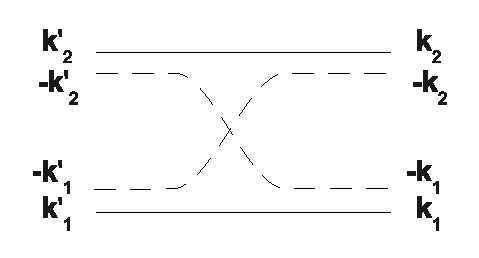
\includegraphics[width=0.3\textwidth]{cobosonCooper/lambda1.eps}\label{fig:lambda}}\qquad
% \subfloat[][]{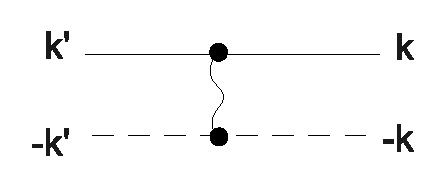
\includegraphics[width=0.3\textwidth]{cobosonCooper/direct1.eps}\label{fig:direct}}\\
%  \subfloat[][]{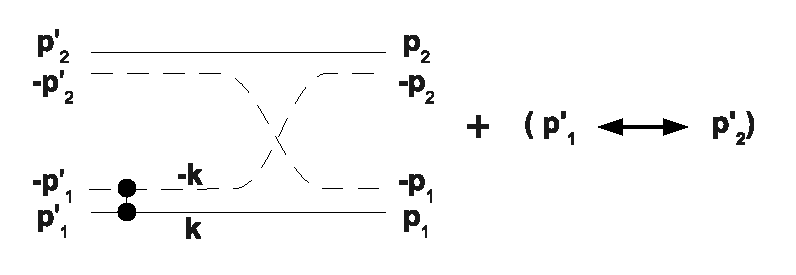
\includegraphics[width=0.4\textwidth]{cobosonCooper/chi1.eps}\label{fig:chi}} 
 \caption{Shiva diagram of free pairs }


 \begin{description}
 
 \item[\subref{fig:lambda}] Pauli scattering $\lambda\fmtrx{\vk'_2}{\vk_2}{\vk'_1}{\vk_1}$ for electron exchange between two free pairs $\br{\vk_1,\vk_2}$, as given by eq. \eqref{eq:pauliscattering}. Up spin electrons are represented by solid line while down spin electrons are represented by dashed line.
 \item[\subref{fig:direct}] The BCS potential given in eq. \eqref{eq:vbcs} transforms a $\vk$ pair into a $\vk'$ pair, with a constant scattering $-V$, in the case of a separable potential $v_{\vk'\vk}=-V\,w_{\vk'}w_{\vk}$. 
 
 \item[\subref{fig:chi}] Interaction scattering  $\chi\fmtrx{\vp'_2}{\vp_2}{\vp'_1}{\vp_1}$ between two free electron pairs, as given in eq \eqref{eq:interactSc}. Since the BCS potential acts within one pair only, the interaction between two pairs can only come from exchange induced by the Pauli exclusion principle.
 \end{description} 


 \end{figure}
\subsection{Fermion interaction}
To get the interaction scatterings associated to fermion interaction, we first note that for a free hamiltonian
\begin{equation}\label{eq:h0}
H_0=\sum{\epsilon_\vk\br{a^{\dagger}_{\vk} a^{}_{\vk}+b^{\dagger}_{\vk} b^{}_{\vk}}}
\end{equation}
Eq. \eqref{eq:aBeta} leads to 
\begin{equation}\label{eq:betaH}
\com{H_0}{\beta^{\dagger}_\vp}=2\epsilon_\vp\beta^{\dagger}_\vp
\end{equation}

We  consider that these fermion pairs interact through the standard BCS like $(1\times1)$ potential in which the fermion $\vk$ only interacts with the fermion $\br{-\vk}$ of the other species. this potential reads
\begin{equation}\label{eq:vbcs}
V_{BCS}=\sum{v_{\vk'\vk}\beta^{\dagger}_{\vk'}\beta^{}_{\vk}}
\end{equation}
It is represented by  the diagram of Fig. \ref{fig:direct}. For this potential, we then have 
\begin{equation}\label{eq:vbeta}
\com{V_{BCS}}{\beta^{\dagger}_\vp}=\gamma^{\dagger}_\vp+V^{\dagger}_\vp
\end{equation}
in which we have $\gamma^{\dagger}_\vp=\sum_\vk\beta^{\dagger}_\vk{}v_{\vk\vp}$. The "creation potential" for the free fermion pair $\vp$ appears to be 
\begin{equation}\label{eq:betaV}
V^{\dagger}_\vp=-{\gamma^{\dagger}_\vp}\br{a^{\dagger}_{\vp}a^{}_{\vp}+b^{\dagger}_{-\vp}b^{}_{-\vp}}
\end{equation}

While the $\gamma^{\dagger}_\vp$ part of eq \eqref{eq:vbcs} commutes with $\beta^{\dagger}_\vp$, this is not so for the creation potential $V^{\dagger}_\vp$.  Its commutator precisely reads
\begin{equation}\label{eq:vpotbeta}
\com{V^{\dagger}_{\vp_1}}{\beta^{\dagger}_{\vp_2}}=-2\delta_{\vp_1\vp_2}\gamma^{\dagger}_{\vp_1}\beta^{\dagger}_{\vp_1}
\end{equation}
This allows us to identify the interaction scattering for free pairs, formally defined as 
\begin{equation}\label{eq:vBeta}
\com{V^{\dagger}_{\vp_1}}{\beta^{\dagger}_{\vp_2}}=\sum\chi\fmtrx{\vp'_2}{\vp_2}{\vp'_1}{\vp_1}\beta^{\dagger}_{\vp'_1}\beta^{\dagger}_{\vp'_2}
\end{equation}
with a sequence of $(2\times2)$ fermion pair exchange and $(1\times1)$ fermion pair interaction. Indeed
\begin{equation}\label{eq:interactSc}
\begin{split}
\chi\fmtrx{\vp'_2}{\vp_2}{\vp'_1}{\vp_1}&=-\sum_\vk\bbr{v_{\vp'_1\vk}\lambda\fmtrx{\vp'_2}{\vp_2}{\vk}{\vp_1}+\br{\vp'_1\leftrightarrow\vp'_2}}\\
&=-\br{v_{\vp'_1,\vp_1}\delta_{\vp'_2,\vp_2}+v_{\vp'_2,\vp_2}\delta_{\vp'_1,\vp_1}}\delta_{\vp_2,\vp_1}
\end{split}
\end{equation}
This interaction scattering is visualized by  the diagram of Fig \ref{fig:chi}: the  free pairs $\vp'_1$ and $\vp'_2$ first exchange a fermion. As for any exchange, this brings a minus sign.  In a second step, the fermions of one of the two pairs interact via the BCS potential.  Note that since the potential has a $(1\times1)$ structure, the $(2\times2)$ interaction between two pairs can only result from fermion exchange, i.e., Pauli blocking. 

We are now going to use this commutation formalism to derive the Richardson equations for Cooper pairs. 

\section{Richardson equations for Cooper pairs\label{sec:rich}}
In order to better grasp how these equations develop, let us  consider an increasing number of pairs. 
\subsection{One pair}
We consider a state in which one free pair $\vk_1$ is added to a frozen Fermi sea $\ket{F_0}$ which does not feel the BCS potential.  This means that the $v_{\vk'\vk}$ prefactors in eq \eqref{eq:vbcs} cancel for all $\vk$ belonging to $\ket{F_0}$.  Note that such a one-pair state actually contains $N_0+1$ fermion pairs, $N_0$ being the number of pairs in the frozen sea.  So that this state is in fact a many-body state, but in the most simple sense since the Fermi sea $\ket{F_0}$ is just there to block states by the Pauli exclusion principle.  It also  brings finite density of state for all the states above it. This is actually crucial to have a bound state, even for an extremely small attracting BCS potential as evidenced below. 

Due to Eqs (\ref{eq:betaH},\ref{eq:vbeta}), the hamiltonian $H=H_0+V_{BCS}$ acting on this one free pair state gives, by taking the zero energy such that $H\ket{F_0}=H_0\ket{F_0}=0$
\begin{equation}
H\beta^{\dagger}_\vk\fo=\com{H}{\beta^{\dagger}_\vk}\fo=\br{2\epsilon_\vk\beta^{\dagger}_\vk+\gamma^{\dagger}_\vk+V^{\dagger}_\vk}\fo
\end{equation}
We then note that, due to the $v_{\vk\vp}$ factor included in the $\gamma^{\dagger}_{\vk}$ part of $V^{\dagger}_\vk$ (see Eq. \ref{eq:betaV}), the creation potential $V^{\dagger}_\vk$ acting on \fo{ }gives zero.

If we now substract $\E_1\beta^{\dagger}_\vk\fo$ to the two sides of the above equation and multiply the result by $\br{2\epsilon_\vk-\E_1}^{-1}$, we find
\begin{equation}\label{eq:HE1}
(H-\E_1)\nth{2\epsilon_\vk-\E_1}\beta^{\dagger}_\vk\fo=\beta^{\dagger}_\vk\fo+\nth{2\epsilon_\vk-\E_1}\sum{}v_{\vk\vp}\beta^{\dagger}_\vp\fo
\end{equation}

To go further and possibly get the one-pair eigenstate of the hamiltonian $H$ in an analytical form, it is necessary to  approximate the BCS potential by a separable potential $v_{\vk\vp}=-V\,w_\vk{}w_\vp$, the $w_\vk$'s being moreover such that $w_\vk^2=w_\vk$.  This yields
\begin{equation}\label{eq:gammaBeta}
\gamma^{\dagger}_\vk=-V\,w_\vk\beta^{\dagger}\quad\quad\beta^{\dagger}=\sum_\vk{}w_\vk\beta^{\dagger}_\vk
\end{equation}
If we then multiply eq \eqref{eq:HE1} by $w_\vk$ and sum over $\vk$, we find
\begin{equation}
(H-\E_1)B^{\dagger}(\E_1)\fo=\br{1-V\sum{\frac{w_\vk}{2\epsilon_\vk-\E_1}}}\beta^{\dagger}\fo
\end{equation}
in which we have set
\begin{equation}\label{eq:B}
B_\vk^{\dagger}(E)=\frac{w_\vk}{2\epsilon_\vk-E}\beta^{\dagger}\quad\quad B^{\dagger}(E)=\sum_\vk{B_\vk^{\dagger}(E)}
\end{equation}
Eq. \eqref{eq:gammaBeta} readily shows that the linear combination  $B^{\dagger}(\E_1)$ of one-pair operators  generates the one-pair eigenstate $B^{\dagger}(\E_1)\fo$ of the hamiltonian $H$ with the energy $\E_1$, provided that this energy is such that
\begin{equation}\label{eq:SchOne}
1=V\sum_\vk{\frac{w_\vk}{2\epsilon_\vk-\E_1}}
\end{equation}
This is nothing but the well-known equation for the single pair energy derived by Cooper.
\subsection{Two pairs}
Let us now consider two pairs.  Eqs. (\ref{eq:betaH},\ref{eq:vbeta})  yield 
\begin{equation}\label{eq:SchTwo}
\begin{split}
H\beta^{\dagger}_{\vk_1}\beta^{\dagger}_{\vk_2}\fo
&=\br{\com{H}{\beta^{\dagger}_{\vk_1}}\beta^{\dagger}_{\vk_2}+\beta^{\dagger}_{\vk_1}\com{H}{\beta^{\dagger}_{\vk_2}}}\fo\\
&=\br{2\epsilon_{\vk_1}+2\epsilon_{\vk_2}}\beta^{\dagger}_{\vk_1}\beta^{\dagger}_{\vk_2}\fo+\ket{v_{\vk_1\vk_2}}
\end{split}
\end{equation}
where $\ket{v_{\vk_1\vk_2}}$ comes from interactions among the $\br{\vk_1,\vk_2}$ pairs induced by the BCS potential.  Its precise value is 
\begin{equation}
\ket{v_{\vk_1\vk_2}}=\br{\gamma^{\dagger}_{\vk_1}\beta^{\dagger}_{\vk_2}+\gamma^{\dagger}_{\vk_2}\beta^{\dagger}_{\vk_1}+V^{\dagger}_{\vk_1}\beta^{\dagger}_{\vk_2}}\fo
\end{equation}
Eq. \eqref{eq:interactSc} allows us to write the last term of $\ket{v_{\vk_1\vk_2}}$ as 
\begin{equation}
V^{\dagger}_{\vk_1}\beta^{\dagger}_{\vk_2}\fo=\com{V^{\dagger}_{\vk_1}}{\beta^{\dagger}_{\vk_2}}\fo=
\sum_{\vp'_1\vp'_2}\chi\fmtrx{\vp'_2}{\vk_2}{\vp'_1}{\vk_1}\beta^{\dagger}_{\vp'_1}\beta^{\dagger}_{\vp'_2}\fo
\end{equation}
So that  $\ket{v_{\vk_1\vk_2}}$ can be visualized by the diagram of Fig. \ref{fig:twoP}. This diagram evidences the fact that, due to the $(1\times1)$ form of the BCS potential, the two pairs $\vk_1$ and $\vk_2$ interact by fermion exchange only, as a result of the Pauli exclusion principle. 

\begin{figure}[htb]
%   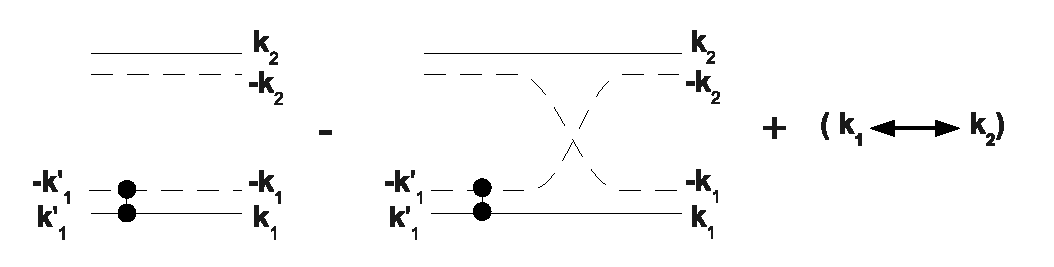
\includegraphics[width=0.4\textwidth]{cobosonCooper/twoPair.eps}
 \caption{Shiva diagram of two pairs \label{fig:twoP}}
\end{figure}

By using the value of the interaction scattering given in Eq. \eqref{eq:vpotbeta},   $\ket{v_{\vk_1\vk_2}}$ is given by
\begin{equation}
\ket{v_{\vk_1\vk_2}}=-V\br{w_{\vk_1}\beta^{\dagger}_{\vk_2}+w_{\vk_2}\beta^{\dagger}_{\vk_1}-2\delta_{\vk_1\vk_2}w_{\vk_1}\beta^{\dagger}_{\vk_1}}\beta^{\dagger}\fo
\end{equation}

To go further, we substract $\E_2\beta^{\dagger}_{\vk_1}\beta^{\dagger}_{\vk_2}\fo$ to the two sides of Eq. \eqref{eq:SchTwo}, with $\E_2$ written as $R_1+R_2$ and we multiply the resulting equation by 
$w_{\vk_1}w_{\vk_2}/\br{2\epsilon_{\vk_1}-R_1}\br{2\epsilon_{\vk_2}-R_2}$. This gives 

\begin{multline}\label{eq:SchTwo2}
(H-\E_2)B^{\dagger}_{\vk_1}(R_1)B^{\dagger}_{\vk_2}(R_2)\fo
=\\
\bbr{B^{\dagger}_{\vk_1}(R_1)\br{w_{\vk_2}\beta^{\dagger}_{\vk_2}-\frac{Vw_{\vk_2}}{2\epsilon_{\vk_2}-R_2}\beta^{\dagger}}
+(1\leftrightarrow2)}\fo
\end{multline}

To go further, we note that $\br{2\epsilon_{\vk_1}-R_1}^{-1}\br{2\epsilon_{\vk_2}-R_2}^{-1}$ also reads  $\mbr{\br{2\epsilon_{\vk_1}-R_1}^{-1}-\br{2\epsilon_{\vk_2}-R_2}^{-1}}/\br{R_1-R_2}$ provided that $R_1\neq{}R_2$. By taking sums over $\vk_1$ and $\vk_2$, Eq. \eqref{eq:SchTwo2} then gives
\begin{multline}\label{eq:SchTwo3}
(H-\E_2)B^{\dagger}(R_1)B^{\dagger}(R_2)\fo
=\\
\bbr{B^{\dagger}(R_1)\br{1-V\sum\frac{w_{\vk}}{2\epsilon_{\vk}-R_2}+\frac{2V}{R_1-R_2}}+(1\leftrightarrow2)}\\
\beta^{\dagger}\fo
\end{multline}
This readily shows that the two-pair state $B^{\dagger}(R_1)B^{\dagger}(R_2)\fo$ is eigenstate of the hamiltonian $H$ with the energy $\E_2=R_1+R_2$ provided that $\br{R_1,R_2}$ fulfill two equations, known as Richardson equations for two pairs.
\begin{equation}
1=V\sum\frac{w_{\vk}}{2\epsilon_{\vk}-R_1}+\frac{2V}{R_1-R_2}=(1\leftrightarrow2)
\end{equation}
\subsection{Three pairs}
We now turn to three pairs to see how these equations develop for an increasing number of pairs. We start with 
\begin{equation}\label{eq:SchThree}
\begin{split}
&H\beta^{\dagger}_{\vk_1}\beta^{\dagger}_{\vk_2}\beta^{\dagger}_{\vk_3}\fo
=\\
&\bbr{\com{H}{\beta^{\dagger}_{\vk_1}}\beta^{\dagger}_{\vk_2}\beta^{\dagger}_{\vk_3}+\beta^{\dagger}_{\vk_1}\com{H}{\beta^{\dagger}_{\vk_2}}\beta^{\dagger}_{\vk_3}+\beta^{\dagger}_{\vk_1}\beta^{\dagger}_{\vk_2}\com{H}{\beta^{\dagger}_{\vk_3}}}\\
&\fo\\
\end{split}
\end{equation}
The same eqs  (\ref{eq:betaH},\ref{eq:vbeta}) give
\begin{equation}\label{eq:SchThree2}
\begin{split}
H\beta^{\dagger}_{\vk_1}\beta^{\dagger}_{\vk_2}\beta^{\dagger}_{\vk_3}\fo
&=\br{2\epsilon_{\vk_1}+2\epsilon_{\vk_2}+2\epsilon_{\vk_3}}\beta^{\dagger}_{\vk_1}\beta^{\dagger}_{\vk_2}\beta^{\dagger}_{\vk_3}\fo\\
&+\ket{v_{\vk_1\vk_2\vk_3}}
\end{split}
\end{equation}
where the part resulting from  the BCS potential appears as 
\begin{equation}\label{eq:vThree}
\begin{split}
\ket{v_{\vk_1\vk_2\vk_3}}=
&\br{\gamma^{\dagger}_{\vk_1}\beta^{\dagger}_{\vk_2}\beta^{\dagger}_{\vk_3}+\gamma^{\dagger}_{\vk_2}\beta^{\dagger}_{\vk_3}\beta^{\dagger}_{\vk_1}+\gamma^{\dagger}_{\vk_3}\beta^{\dagger}_{\vk_1}\beta^{\dagger}_{\vk_2}}\fo\\
&+\br{V^{\dagger}_{\vk_1}\beta^{\dagger}_{\vk_2}\beta^{\dagger}_{\vk_3}+\beta^{\dagger}_{\vk_1}V^{\dagger}_{\vk_2}\beta^{\dagger}_{\vk_3}+\beta^{\dagger}_{\vk_1}\beta^{\dagger}_{\vk_2}V^{\dagger}_{\vk_3}}\fo
\end{split}
\end{equation}
The last term  gives zero since $V^{\dagger}_\vk\fo=0$.  Using Eq. \eqref{eq:vBeta}, the two remaining terms of the second bracket can be rewritten as 
\begin{equation}\label{eq:vThree2}
\begin{split}
&\bbr{\com{V^{\dagger}_{\vk_1}}{\beta^{\dagger}_{\vk_2}}\beta^{\dagger}_{\vk_3}+\beta^{\dagger}_{\vk_2}\com{V^{\dagger}_{\vk_1}}{\beta^{\dagger}_{\vk_3}}+\beta^{\dagger}_{\vk_1}\com{V^{\dagger}_{\vk_2}}{\beta^{\dagger}_{\vk_3}}}\fo\\
=&\sum_{vk'_1\vk'_2}\beta^{\dagger}_{\vk'_1}\beta^{\dagger}_{\vk'_2}\\
&\bbr{\chi\fmtrx{\vk'_2}{\vk_2}{\vk'_1}{\vk_1}\beta^{\dagger}_{\vk_3}+\chi\fmtrx{\vk'_2}{\vk_3}{\vk'_1}{\vk_2}\beta^{\dagger}_{\vk_1}+\chi\fmtrx{\vk'_2}{\vk_1}{\vk'_1}{\vk_3}\beta^{\dagger}_{\vk_2}}\fo
\end{split}
\end{equation}
This leads to represent the vector $\ket{v_{\vk_1\vk_2\vk_3}}$ by the diagram of Fig. \ref{fig:threeP}. This interaction term results from  interactions inside a single pair, with in addition  a possible exchange with a second pair, the third pair then staying unchanged. 
\begin{figure}[htb]
%   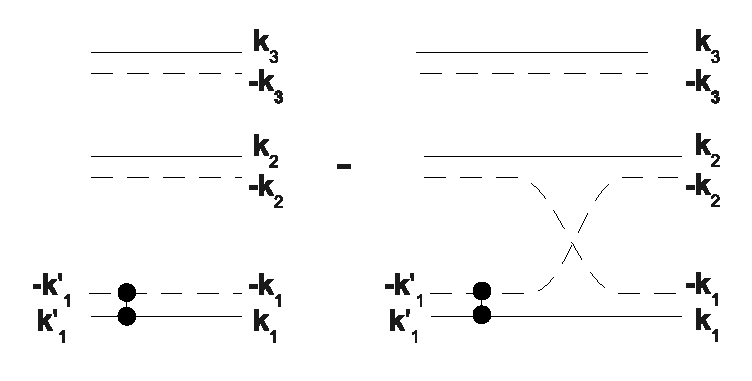
\includegraphics[width=0.4\textwidth]{cobosonCooper/threePair.eps}
 \caption{Shiva diagram of two pairs \label{fig:threeP}}
Part resulting from the BCS potential acting on three pairs, as given in Eqs. (\ref{eq:vThree},\ref{eq:vThree2}). $\ket{v_{\vk_1\vk_2\vk_3}}$ also contains two similar contributions as the one visualized in this figure, obtained by circular permutation. 
\end{figure}

If we come back to Eq. \eqref{eq:SchThree2}, substract $\E_3\beta^{\dagger}_{\vk_1}\beta^{\dagger}_{\vk_2}\beta^{\dagger}_{\vk_3}\fo$ to both sides, with $\E_3$ written as $R_1+R_2+R_3$, and multiply the resulting equation by $w_{\vk_1}w_{\vk_2}w_{\vk_3}/\br{2\epsilon_{\vk_1}-R_1}\br{2\epsilon_{\vk_2}-R_2}\br{2\epsilon_{\vk_3}-R_3}$, we find

\begin{multline}\label{eq:SchThree3}
(H-\E_3)B^{\dagger}_{\vk_1}(R_1)B^{\dagger}_{\vk_2}(R_2)B^{\dagger}_{\vk_3}(R_3)\fo=\\
\bbr{B^{\dagger}_{\vk_1}(R_1)B^{\dagger}_{\vk_2}(R_2)\br{w_{\vk_3}\beta^{\dagger}_{\vk_3}-\frac{Vw_{\vk_3}}{2\epsilon_{\vk_2}-R_3}\beta^{\dagger}}+\text{2 perm}}\\\fo\\
+2V\bbr{B^{\dagger}_{\vk_3}(R_3)\frac{\delta_{\vk_1\vk_2}w_{\vk_1}}{\br{2\epsilon_{\vk_1}-R_1}\br{2\epsilon_{\vk_1}-R_2}}\beta^{\dagger}_{\vk_1}+\text{2 perm}}\\\beta^{\dagger}\fo
\end{multline}
To proceed, we rewrite  $\br{2\epsilon_{\vk_1}-R_1}^{-1}\br{2\epsilon_{\vk_2}-R_2}^{-1}$  as 
$\mbr{\br{2\epsilon_{\vk_1}-R_1}^{-1}-\br{2\epsilon_{\vk_2}-R_2}^{-1}}/\br{R_1-R_2}$ provided that $R_1\neq{}R_2$ and do the same for the two other products. By taking the sum over $\br{\vk_1,\vk_2,\vk_3}$, we end with 

\begin{multline}\label{eq:SchThree4}
(H-\E_3)B^{\dagger}(R_1)B^{\dagger}(R_2)B^{\dagger}(R_3)\fo=\\
\{B^{\dagger}(R_2)B^{\dagger}(R_3)\\
\br{1-V\sum\frac{w_{\vk_1}}{2\epsilon_{\vk_1}-R_1}-\frac{2V}{R_1-R_2}+\frac{2V}{R_3-R_1}}\\+\text{2 perm}\}\beta^{\dagger}\fo
\end{multline}

This leads us to again conclude that the three-pair state $B^{\dagger}(R_1)B^{\dagger}(R_2)B^{\dagger}(R_3)\fo$ is eigenstate of the hamiltonian with the energy $\E_3=R_1+R_2+R_3$, provided that $\br{R_1,R_2, R_3}$ fulfill the three equations, 
\begin{equation}
\begin{split}
1&=V\sum\frac{w_{\vk}}{2\epsilon_{\vk}-R_1}+\frac{2V}{R_1-R_2}+\frac{2V}{R_1-R_3}\\
1&=V\sum\frac{w_{\vk}}{2\epsilon_{\vk}-R_2}+\frac{2V}{R_2-R_3}+\frac{2V}{R_2-R_1}\\
1&=V\sum\frac{w_{\vk}}{2\epsilon_{\vk}-R_3}+\frac{2V}{R_3-R_1}+\frac{2V}{R_3-R_2}
\end{split}
\end{equation}

\subsection{N pairs}
The above commutation technique can be easily generated to N pairs. As nicely visualized by the diagrams of Figs. \ref{fig:twoP} and \ref{fig:threeP}, the effect of the BCS potential on these N pairs splits into two sets of terms: In one set, one pair is affected by the $(1\times1)$ scattering while the other $N-1$ pairs stay unchanged. In the other, this pair in addition has a fermion exchange before the interaction, with an other pair, the remaining $N-2$ pairs staying unchanged. This readily shows that to increase the  number of pairs above two, does not really change the structure of the equations since $N-2$ pairs stay unchanged, the pair exchanging its fermions using the pair suffering the interaction  being just one among $(N-1)$ pairs. 

Although the equations become more and more cumbersome to be explicitly written, the procedure is rather straight-forward once we have understood that either $(N-1)$ or $(N-2)$ pairs stay unaffected in the process.  The general form of the N-pair eigenstate ultimately appears as 
\begin{equation}\label{eq:SchThreeN}
(H-\E_N)B^{\dagger}(R_1)\cdots{}B^{\dagger}(R_N)\fo=0
\end{equation}
with $\E_3=R_1+\cdots+R_N$, these $R_N$'s being  solutions of $N$ equations like
\begin{equation}
1=V\sum\frac{w_{\vk}}{2\epsilon_{\vk}-R_i}+\sum_{i\neq{j}}\frac{2V}{R_i-R_j}\quad\qquad \text{for}\; i=\br{1,...,N}
\end{equation}

\subsection{Physical understanding}
This new derivation of the Richardson equation has the main advantage to possibly trace back the parts in these equations which are directly linked to the Pauli exclusion principle between fermion pairs. 

From a mathematical point of view, the link is rather obvious: In the absence of terms like $(R_i-R_j)$, the $N$ equations for $R_i$ reduced to the same equation \eqref{eq:SchOne}, so that the result would be $R^0_i=\E_1$ for all $i$.  The fact that the energy of $N$ pairs differs from $N$ times the single pair energy thus comes from those $(R_i-R_j)$ differences. 

Physically, the fact that $\E_N$ differs from $N\E_1$ comes from interactions between pairs. Due to the $(1\times1)$ form of the BCS potential, interaction between pairs can only be mediated by fermion exchanges as clear from Fig. \ref{fig:chi}.  Interaction between pairs thus is solely the result of the Pauli exclusion principle between pairs. This Pauli blocking mathematically appears through the various $\delta_{\vp'\vp}$ factors appearing in Pauli scatterings 
$\lambda\fmtrx{\vp'_2}{\vp_2}{\vp_1'}{\vp_1}$.  It is then easy to mathematically trace back the  $(R_i-R_j)$ differences appearing in the Richardson equations to these $\delta$ factors. 

In short, the Kronecker symbols in the Pauli scatterings of  fermion pairs result from the Pauli exclusion principle.  They induce terms with $(R_i-R_j)$ differences in the Richardson equations which make the energy of $N$ pairs different from the one of a collection of $N$ independent single pairs. 

Another very interesting feature of the energy $\E_N$ of $N$ pairs, this new derivation explains in a rather clear way, is the fact that the part of the $N$ pairs energy coming from interaction, namely $\E_N-N\E_1$ depends on $N$ as $N(N-1)$ only. Indeed, diagram \ref{fig:threeP} evidences that the contribution of the $(1\times1)$ BCS potential mixed with fermion exchanges between pairs having one degree of freedom only, ends by producing effective scatterings which are $(2\times2)$ only.  Since, in order to have terms in $N(N-1)(N-2)$, we need topologically connected interaction processes between 3 objects, $N(N-1)(N-2)$ terms as well as all the higher order terms, cannot exist in the energy of $N$ Cooper pairs.

This actually is what we have found by solving these equations analytically in the dilute limit on the single Cooper pair scale.   In this limit, the energy of N pairs was shown to read as 
\begin{equation}\label{eq:en}
\E_N=N\E_1+N(N-1)\br{\nth{\rho_0}+\frac{\epsilon_c}{N_\Omega}}
\end{equation}
$\rho_0$ is the density of pair states in the potential layer, $N_\Omega=\rho_0\Omega$ is number of states in the layer, and $\epsilon_c$ is the single pair binding energy.  By writing it as $\epsilon_c=N_\Omega\epsilon_V$, this energy also reads, for $\E_1=2\epsilon_{F_0}-\epsilon_c$ where $\epsilon_{F_0}$ is the Fermi level of the frozen sea \fo
\begin{equation}
\E_N=2N\mbr{\epsilon_{F_0}+\frac{N(N-1)}{\rho_0}}-N\epsilon_V\br{N_V-\frac{N-1}{N_\Omega}}
\end{equation}
The first term corresponds to the kinetic energy of $N$ pairs added to $\epsilon_{F_0}$, i.e., 
\begin{equation}
2\efo+\br{2\efo+1/\rho_0}+\cdots\;+\br{2\efo+(N-1)/\rho_0}
\end{equation}
The second term evidences the fact that the Cooper pair binding energy linearly decreases with pair number, this energy being proportional to the number of empty states $N_V-(N-1)$ filling the potential.  

This brings the binding energy down to $\epsilon_c/2$ in the BCS configuration, i.e., when pairs fill half the potential layer. Actually, the result  fully agrees with the BCS condensation energy, ??? to read
\begin{equation}
E_{\text{super}}-E_\text{normal}=\nth{2}\rho_0\Delta^2=\frac{\rho_0\Omega}{2}\frac{2\Omega{e^{-2/\rho_0V}}}{2}
\end{equation}
In spite of the fact that Eq. \eqref{eq:en} has up to now been derived within the dilute limit only, it turns out that it is valid over the whole density range.  This validity is a bare result of the existence of $(2\times2)$ effective scatterings only between fermion pairs, this argument having nothing to do with the pair density large or small on the single Cooper pair scale. 

\section{Richardson exact eigenstate versus BCS ansatz \label{sec:conn}}
Another very interesting result the Richardson procedure generates is the \emph{exact} form of the eigenstate, namely
\begin{equation}
B^{\dagger}(R_1)\cdots{}B^{\dagger}(R_N)\fo
\end{equation}
with $B^{\dagger}(R)$ given by Eq. \eqref{eq:B}.  The fact that by construction all the $R_i$'s are different, strongly questions the standard BCS ansatz. For Cooper pair wave function $\br{B^{\dagger}}^N\fo$ with \emph{all} the pairs condensed into the same state. 

To discuss this problem on precise grounds, let us start with two pairs.  In a previous work\cite{combescotBCS}, we have shown, that the two "Richardson energies" then read $R_1=R+iR'$ and $R_2=R-i{}R'$ with $R$ and $R'$ real, their precise values being $R\approx\epsilon_c+1/\rho_0+\epsilon_c/N\Omega$ and $R'=\sqrt{2\epsilon_c/\rho_0}$ in the large sample limit, i.e. for $1/\rho_0$ small.  By noting that
\begin{multline}
B^{\dagger}(R_1)B^{\dagger}(R_2)=\\
\mbr{B^{\dagger}(R)+B^{\dagger}(R_1)-B^{\dagger}(R)}\mbr{B^{\dagger}(R)+B^{\dagger}(R_2)-B^{\dagger}(R)}
\end{multline}
we get from eq \eqref{eq:B}
\begin{equation}
B^{\dagger}(R_1)B^{\dagger}(R_2)=\mbr{B^{\dagger}(R)}^2+R'^2\bbr{C^{\dagger}_+C^{\dagger}_--2B^{\dagger}(R)D^{\dagger}}
\end{equation}
where we have set 
\begin{align}
C^{\dagger}_{\pm}&=\sum\frac{w_\vk}{\br{2\epsilon_\vk-R}\br{2\epsilon_\vk-R\pm{}iR'}}\beta^{\dagger}_\vk\\
D^{\dagger}&=\sum\frac{w_\vk}{\br{2\epsilon_\vk-R}\mbr{\br{2\epsilon_\vk-R}^2+{}R'^2}}\beta^{\dagger}_\vk
\end{align}
So that at first order in sample volume, i.e., in $1/\rho_0$, we  find since $N_\Omega=\rho_0\Omega$
\begin{multline}\label{eq:BB}
B^{\dagger}(R_1)B^{\dagger}(R_2)-\mbr{B^{\dagger}(\frac{\E_2}{2})}^2\approx
\frac{2\epsilon_c}{\rho_0}\\\bbr{-2B^{\dagger}(\E_1)\sum\frac{w_\vk}{\br{2\epsilon_\vk-\E_1}^3}\beta^{\dagger}_\vk
+\mbr{\sum\frac{w_\vk}{\br{2\epsilon_\vk-\E_1}^2}\beta^{\dagger}_\vk}^2}\\+O(\nth{\rho_0^2})
\end{multline}
The above result shows that $B^{\dagger}(R_1)B^{\dagger}(R_2)$ can be written as $\br{B^{\dagger}(\E_2/2)}^2$ provided that we drop all $1/\rho_0$ terms.  However $B^{\dagger}$ then reduces to $B^{\dagger}(\E_1)$.  This barely corresponds to consider the two-pair eigenstate as the product of two non-interacting single pairs.  If instead, we want, in the condensed pair creation operator, include the change from one to two pairs induced by Pauli blocking which brings the energy per pair from $\E_1$ to $\E_2/2=\E_1+1/\rho_0+\epsilon_c/N_\Omega$, we are led to replace $B^{\dagger}(R_1)B^{\dagger}(R_2)$ by $\br{B^{\dagger}(\E_2/2)}^2$.  This however is inconsistent because we then keep in this condensed pair operator, contribution in $1/\rho_0$ which are as large as the ones we drop in the LHS of eq \eqref{eq:BB}.  In the case of two pairs, the replacement of the exact eigenstate  $B^{\dagger}(R_1)B^{\dagger}(R_2)\fo$ by a BCS-like condense state $\br{B^{\dagger}(\E_2/2)}^2\fo$ thus is inconsistent. 

It is actually claimed that the BCS ansatz is valid in the thermodynamical limit, i.e., for $N$ and $V$ both very large.  Derivation of the "validity" is in fact with restrict to the energy only. We fully agree that the BCS ansatz give the correct energy since the energy obtained using this ansatz is just the one we have derived from the exact Richardson procedure.  However agreement on the energy by no mean proves agreement on the wave function. Many examples have been given in the past with wave function very different from the exact one, while giving the correct energy.  

The possible replacement of $B^{\dagger}(R_1)\cdots{}B^{\dagger}(R_N)\fo$ by $\br{B^{\dagger}}^N\fo$ is actually crucial to support the overall picture we all have of superconductivity, with all the pairs in the same state, as an army of little solders, all walking similarly.  

This question of the BCS ansatz in the wave function has the approached in a different way by Bogoliubox.  Let us here reconsider his argument.  

\section{Conclusion}
We have rederived the Richardson equations using a commutation technique for free electron pairs with zero total momentum similar to the one we have developed for composite boson excitons.  Almost half a century ago, Richardson has shown that the \emph{exact} wave-function and energy for an arbitrary number $N$ of pairs can be written in a compact form in terms of $N$ energy-like quantities $R_1,..., R_N$, which are solution of $N$ coupled non-linear equations.  This $2N$ many-body problem is exactly solvable provided that the interaction potential is taken as a BCS-like $\abs{x}$ potential having a separable scattering $v_{\vk'\vk}=-V\,w_{\vk'}w_{\vk}$ with $w_{\vk}$ ?????? such that $w_\vk^2=1$.  Note that these assumptions are already those necessary to get the energy of a single pair in the compact form obtained by Cooper.  Richardson manged to extend this exact solution to $N$ pairs by decoupling them through rewriting their energy $E_N$ as $R_1+\cdots+R_N$.

The new composite boson derivation we have proposed allows to trace back the physical origin of the various terms of these equations.  It in particular clearly shows that $N$ pairs differ from $N$ independent single pairs, due to Pauli exclusion principle only.  This Pauli blocking also enforces the $R_i$ energy-like parameters to be different, namely the exact $N$-pair eigenstate different from the BCS ansatz.  ?????? the diagrammatic representation of this derivation evidences that, due to the fact that pairs with zero total momentum, do have one degree of freedom only, they only have $2\times2$ scatterings within the $1\times1$ BCS potential. This explains why the $N$ pair energy has terms in $N$ and $N(N-1)$ but not in $N(N-1)(N-2)$ and so on.

One of us (M.C.) wishes to thank the Institute of Condensed Matter Physics of the University of Illinois, Urbana-Champaign, and Tony Leggett in particular, for her one-month invitation.  

\begin{thebibliography}{6}
\expandafter\ifx\csname natexlab\endcsname\relax\def\natexlab#1{#1}\fi
\expandafter\ifx\csname bibnamefont\endcsname\relax
  \def\bibnamefont#1{#1}\fi
\expandafter\ifx\csname bibfnamefont\endcsname\relax
  \def\bibfnamefont#1{#1}\fi
\expandafter\ifx\csname citenamefont\endcsname\relax
  \def\citenamefont#1{#1}\fi
\expandafter\ifx\csname url\endcsname\relax
  \def\url#1{\texttt{#1}}\fi
\expandafter\ifx\csname urlprefix\endcsname\relax\def\urlprefix{URL }\fi
\providecommand{\bibinfo}[2]{#2}
\providecommand{\eprint}[2][]{\url{#2}}

\bibitem[{\citenamefont{Bardeen et~al.}(1957)\citenamefont{Bardeen, Cooper, and
  Schrieffer}}]{BCS}
\bibinfo{author}{\bibfnamefont{J.}~\bibnamefont{Bardeen}},
  \bibinfo{author}{\bibfnamefont{L.~N.} \bibnamefont{Cooper}},
  \bibnamefont{and} \bibinfo{author}{\bibfnamefont{J.~R.}
  \bibnamefont{Schrieffer}}, \bibinfo{journal}{Physical Review}
  \textbf{\bibinfo{volume}{106}}, \bibinfo{pages}{162} (\bibinfo{year}{1957}).

\bibitem[{\citenamefont{Richardson}(1963)}]{Richardson1}
\bibinfo{author}{\bibfnamefont{R.~W.} \bibnamefont{Richardson}},
  \bibinfo{journal}{physics letters} \textbf{\bibinfo{volume}{3}},
  \bibinfo{pages}{277} (\bibinfo{year}{1963}).

\bibitem[{\citenamefont{Richardson and Sherman}(1964)}]{Richardson2}
\bibinfo{author}{\bibfnamefont{R.~W.} \bibnamefont{Richardson}}
  \bibnamefont{and} \bibinfo{author}{\bibfnamefont{N.}~\bibnamefont{Sherman}},
  \bibinfo{journal}{Nucl. Phys.} \textbf{\bibinfo{volume}{52}},
  \bibinfo{pages}{221} (\bibinfo{year}{1964}).

\bibitem[{\citenamefont{Combescot et~al.}(2008)\citenamefont{Combescot,
  Betbeder-Matibet, and Dubin}}]{CobosonPhysicsReports}
\bibinfo{author}{\bibfnamefont{M.}~\bibnamefont{Combescot}},
  \bibinfo{author}{\bibfnamefont{O.}~\bibnamefont{Betbeder-Matibet}},
  \bibnamefont{and} \bibinfo{author}{\bibfnamefont{F.}~\bibnamefont{Dubin}},
  \bibinfo{journal}{Physics Reports} \textbf{\bibinfo{volume}{463}},
  \bibinfo{pages}{215} (\bibinfo{year}{2008}).

\bibitem[{\citenamefont{Combescot and
  Betbeder-Matibet}(2007)}]{CobosonCalculation}
\bibinfo{author}{\bibfnamefont{M.}~\bibnamefont{Combescot}} \bibnamefont{and}
  \bibinfo{author}{\bibfnamefont{O.}~\bibnamefont{Betbeder-Matibet}},
  \bibinfo{journal}{The European Physical Journal B}
  \textbf{\bibinfo{volume}{55}}, \bibinfo{pages}{63} (\bibinfo{year}{2007}).

\bibitem[{\citenamefont{Pogosov1 et~al.}()\citenamefont{Pogosov1, Combescot,
  and Crouzeix}}]{combescotBCS}
\bibinfo{author}{\bibfnamefont{W.~V.} \bibnamefont{Pogosov1}},
  \bibinfo{author}{\bibfnamefont{M.}~\bibnamefont{Combescot}},
  \bibnamefont{and} \bibinfo{author}{\bibfnamefont{M.}~\bibnamefont{Crouzeix}}.

\end{thebibliography}

\end{document}
